\chapter{Cirrhosis}
\label{applications-efx_country_level}

Fixed effects can also increase the accuracy of out-of-sample predictions.  By modeling the relationship between the epidemiologic parameter of interest and the explanatory covariate, extrapolation can predict for epidemiologic parameters in areas where no epidemiologic parameter measurements are available but covariate data are.  Few regions have epidemiologic measurements for cirrhosis.  However, by using the age-standardized hepatitis C prevalence as a country-level covariate to predict out-of-sample, it is possible to estimate the prevalence of cirrhosis.

The result of chronic liver injury, cirrhosis is an advanced stage of liver scarring.  Cirrhosis is the end stage of any chronic liver disease, with the most common causes being alcoholic liver disease and hepatitis B and C.  Asymptomatic during the early stages of the disease, compensated cirrhosis may go undetected until complications develop.  The diagnostic gold standard for cirrhosis is a liver biopsy.  Complications such as portal hypertension, jaundice, ascites, gastrointestinal bleeding and liver dysfunction mark the progression from compensated to decompensated cirrhosis.  Irreversible, cirrhosis management is the prevention, control and treatment of cirrhosis complications, with liver transplantation being the ultimate treatment.  Without a liver transplant, cirrhosis mortality is very high \cite{garcia-tsao_management_2009, d'amico_natural_2006, schuppan_liver_2008}.

Systematic review yielded prevalence, excess mortality  rate estimates from four (of 21 possible) regions.  Given the difficulty in cirrhosis diagnosis, it is assumed this data represents decompensated cirrhosis and the following analysis focuses on the decompensated phase of the disease, assuming almost all prevalent cases lead to death.

    \begin{figure}[h]
        \begin{center}
            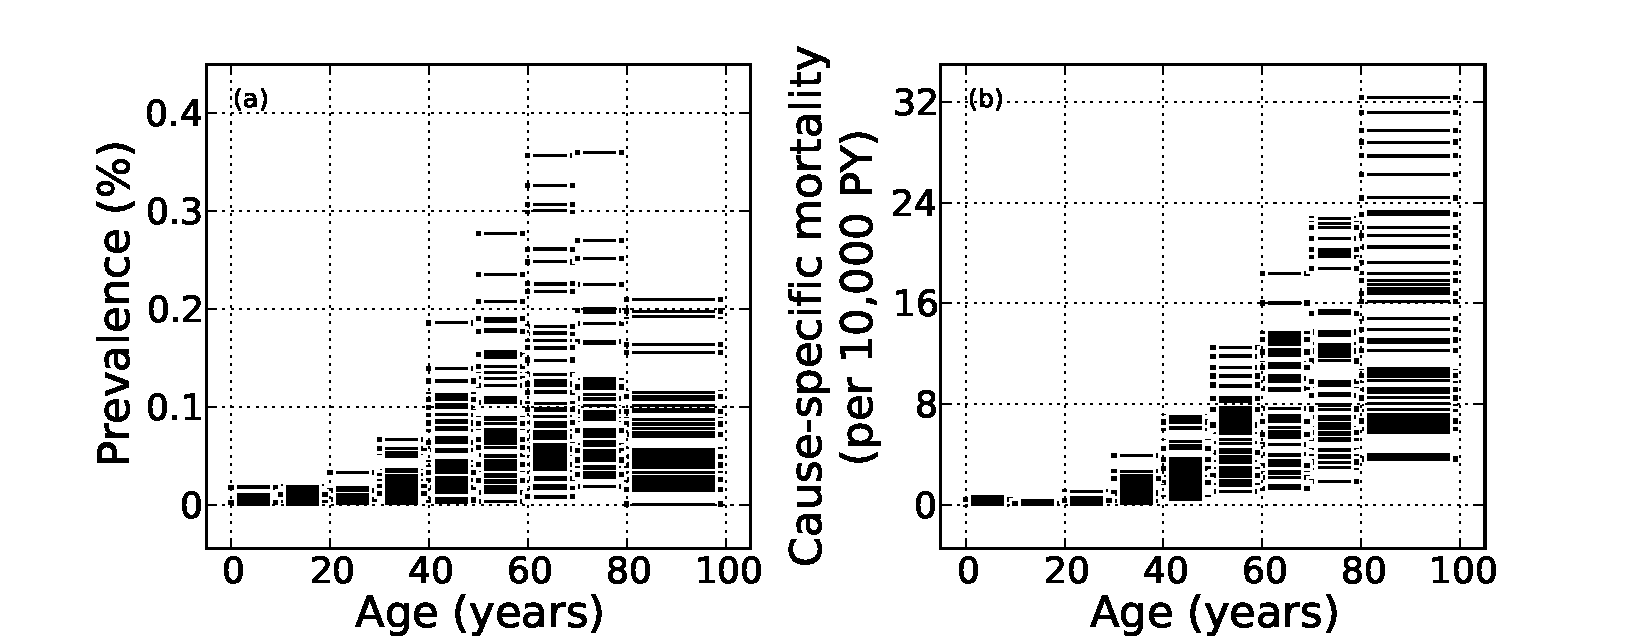
\includegraphics[width=\textwidth]{cirrhosis-data.pdf}
            \caption{Available global data for cirrhosis prevalence and pf.}
            \label{fig:app-cirrhosis data}
        \end{center}
    \end{figure}
    
    
    
borrow strength from the mortality estimates to inform the incidence estimates
using estimates of age-standardized hepatitis C prevalence as an explanatory covariate for estimating the prevalence of cirrhosis�.???
    